%%%%%%%%%%%%%%%%%%%%%%%%%%%%%%%%%%%%%%%%%
% Journal Article
% LaTeX Template
% Version 1.4 (15/5/16)
%
% This template has been downloaded from:
% http://www.LaTeXTemplates.com
%
% Original author:
% Frits Wenneker (http://www.howtotex.com) with extensive modifications by
% Vel (vel@LaTeXTemplates.com)
%
% License:
% CC BY-NC-SA 3.0 (http://creativecommons.org/licenses/by-nc-sa/3.0/)
%
%%%%%%%%%%%%%%%%%%%%%%%%%%%%%%%%%%%%%%%%%

\documentclass[twoside,twocolumn]{article}

%----------------------------------------------------------------------------------------
%	PACKAGES AND OTHER DOCUMENT CONFIGURATIONS
%----------------------------------------------------------------------------------------

\usepackage{blindtext} % Package to generate dummy text throughout this template 

\usepackage[sc]{mathpazo} % Use the Palatino font
\usepackage[T1]{fontenc} % Use 8-bit encoding that has 256 glyphs
\linespread{1.05} % Line spacing - Palatino needs more space between lines
\usepackage{microtype} % Slightly tweak font spacing for aesthetics

\usepackage[german]{babel} % Language hyphenation and typographical rules

\usepackage[hmarginratio=1:1,top=32mm,columnsep=20pt]{geometry} % Document margins
\usepackage[hang, small,labelfont=bf,up,textfont=it,up]{caption} % Custom captions under/above floats in tables or figures
\usepackage{booktabs} % Horizontal rules in tables

\usepackage{lettrine} % The lettrine is the first enlarged letter at the beginning of the text

\usepackage{enumitem} % Customized lists
\setlist[itemize]{noitemsep} % Make itemize lists more compact

\usepackage{abstract} % Allows abstract customization
\renewcommand{\abstractnamefont}{\normalfont\bfseries} % Set the "Abstract" text to bold
\renewcommand{\abstracttextfont}{\normalfont\small\itshape} % Set the abstract itself to small italic text

\usepackage{titlesec} % Allows customization of titles
\renewcommand\thesection{\Roman{section}} % Roman numerals for the sections
\renewcommand\thesubsection{\roman{subsection}} % roman numerals for subsections
\titleformat{\section}[block]{\large\scshape\centering}{\thesection.}{1em}{} % Change the look of the section titles
\titleformat{\subsection}[block]{\large}{\thesubsection.}{1em}{} % Change the look of the section titles

\usepackage{fancyhdr} % Headers and footers
\pagestyle{fancy} % All pages have headers and footers
\fancyhead{} % Blank out the default header
\fancyfoot{} % Blank out the default footer
\fancyhead[C]{Ressourcenoptimierung im E-Commerce, mittels KI $\bullet$ May 2022 $\bullet$ Vol. I, No. 1} % Custom header text
\fancyfoot[RO,LE]{\thepage} % Custom footer text

\usepackage{titling} % Customizing the title section

\usepackage{hyperref} % For hyperlinks in the PDF

\usepackage{graphicx}

\parindent0cm
%----------------------------------------------------------------------------------------
%	TITLE SECTION
%----------------------------------------------------------------------------------------

\setlength{\droptitle}{-4\baselineskip} % Move the title up

\pretitle{\begin{center}\Huge\bfseries} % Article title formatting
	\posttitle{\end{center}} % Article title closing formatting
\title{Ressourcenoptimierung im E-Commerce, durch den Einsatz von künstlicher Intelligenz.} % Article title
\author{%
	\textsc{Wilfried Pahl}%\thanks{A thank you or further information} \\[1ex] % Your name
	\normalsize Berliner Hochschule für Technik \\ % Your institution
	\normalsize \href{mailto:s81179@beuth-hochschule.de}{s81179@beuth-hochschule.de} % Your email address
	%\and % Uncomment if 2 authors are required, duplicate these 4 lines if more
	%\textsc{Jane Smith}\thanks{Corresponding author} \\[1ex] % Second author's name
	%\normalsize University of Utah \\ % Second author's institution
	%\normalsize \href{mailto:jane@smith.com}{jane@smith.com} % Second author's email address
}
\date{\today} % Leave empty to omit a date


%----------------------------------------------------------------------------------------


\renewcommand{\maketitlehookd}{
	\begin{abstract}
		Die künstliche Intelligenz hat in vielen Bereichen der digitalen Einzug gehalten. Großen Potenzial, für die künstliche Intelligenz gibt es auch im Bereich des E-Commerce. Durch die Einführung von künstlicher Intelligenz wird gezeigt wie Prozesse im E-Commerce optimiert und dadurch Ressourcen eingespart werden. Bei den hier aufgezeigten Lösungen konnten die Kosten für Personal, Lagerhaltung und Werbemittel um 35\% gesenkt werden, bei einem Mehraufwand an Investitionskosten von 5\% des monatlichen Umsatzes, für neue Technologie und deren Einführung.
	\end{abstract}
}

\begin{document}
	
	% Print the title
	\maketitle
	
	%----------------------------------------------------------------------------------------
	%	ARTICLE CONTENTS
	%----------------------------------------------------------------------------------------
	
	\section{Einleitung}
	Optimierung der Ressourcen ist ein wichtiger Teil, um im hart umkämpften Markt der Onlinehändler konkurrenzfähig zu bleiben. Um eine Reduzierung des Ressourcenverbrauchs zu bewirken, müssen die Prozesse im Onlinehandel analysiert und automatisiert werden. Künstliche Intelligenz kann nicht nur einfache Aufgaben übernehmen und die Ressourcen einsparen, sondern senkt auch die Fehlerquote bei der Abarbeitung dieser Aufgaben.\vspace{0.2cm}

Sollen die Prozesse optimal erfasst werden, ist es essenziell, dass die Mitarbeiter des Onlinehandels frühzeitig in die Prozessoptimierung eingebunden und ihnen klar wird, dass sie nicht überflüssig werden, sondern an anderen Stellen im Handel eingesetzt werden. Wir betrachten ein Beispiel einer E-Commerce-Plattform, die neben dem eigentlichen Shop über einen eigenen Lieferservice und über eigene Abteilungen zur Vermarktung und Kundenbetreuung verfügt. Diese Plattform hat künstliche Intelligenz für die Prozessoptimierung eingeführt.\vspace{0.2cm}

Ich werde die Erhebung und Verwendung der Daten bewerten, die für den Einsatz von künstlicher Intelligenz erforderlich sind, um die Prozesse zu optimieren. Ebenfalls wird eine mögliche Systemlandschaft vorgestellt, um die erforderliche Infrastruktur bereit zustellen. In dieser Systemlandschaft wird die künstliche Intelligenz optimal eingesetzt und eine Optimierung einzelner Komponenten kann nach Bedarf erfolgen.\vspace{0.2cm}

Ich betrachte in dieser Arbeit drei Bereiche \textit{Planung und Prozess}, \textit{Produktangebot und -darstellung} sowie \textit{Beratung und Service}. In alles drei Bereichen werden Lösungen aufgezeigt, die die Prozesse teilweise oder voll automatisieren und somit zur Ressourcenoptimierung beitragen. Der Bereich \textit{Planung und Prozess} zeigt Lösungen, die Prozesse des E-Commerce optimiert. Hier werden Technologien eingesetzt, die Prozesse optimieren, die neben dem eigentlichen Onlinegeschäft liegen. Dies sind Prozesse der Bedarfsermittlung, Lagerverwaltung und Liefermanagement. Prozesse, die für die Kundenneugewinnung optimiert werden, finden sich im Bereich der \textit{Produktangebote und -darstellung} wieder. Die hier eingesetzten Technologien, die mithilfe der künstlichen Intelligenz gesteuert und überwacht werden, übernehmen Aufgaben der Webseiten- und Produktgestaltung. Ebenso werden Methoden zur Vorhersage und optimierten Anzeigen möglicher benötigter Produkte verwendet. Bleibt noch der Bereich \textit{Beratung und Service}. Die hier eingesetzten Methodiken und Technologien unterstützen Prozesse zur Kundengewinnung und -betreuung. Auch Prozesse zur Kundenrückgewinnung werden betrachtet. Alle Optimierungen für das Kundenmanagement unterstützen dabei, die Arbeitsaufwände der Mitarbeiter zu reduzieren. Somit werden Mitarbeiterressourcen freigesetzt, die beispielsweise im Kundendienst anspruchsvollere Aufgaben übernehmen können.\vspace{0.2cm}

Um die Optimierung zu demonstrieren, werden folgende Lösungen gezeigt,

\begin{enumerate}[label=(\arabic*)]
	\item Es wird gezeigt wie künstliche Intelligenz dazu beträgt die Ressourcen im Onlinehandel einzusparen.
	\item Ich schlage Technologien vor, welche die Kundenzufriedenheit steigern und somit zur Umsatzsteigerung beitragen.
	\item Es wird gezeigt, dass durch den Einsatz von künstlicher Intelligenz die Mitarbeiterzufriedenheit steigt, weil diese jetzt anspruchsvollere Aufgaben übernehmen und durch erhöhte Motivation zur Umsatzsteigerung beitragen.
\end{enumerate}

	\section{Künstliche Intelligenz im E-Commerce}
	Eine künstliche Intelligenz kann anhand von aktuellen Nutzerdaten und Statistiken von gesammelten Daten viele Aufgaben aus dem Bereich des Online-Handels übernehmen. Hinzu kommen äußere Faktoren wie Tageszeit, Tage vor Feiertage, Geographische Lage, aktuelle Trends oder Jahreszeit\vspace{0.2cm}

Bereits bei der Generierung der Produktpräsentation kann die künstliche Intelligenz personalisierte Produkte  bereitstellen und den Aufbau des Onlineshop an das Verhalten des Nutzers anpassen. Somit wird das gesamte ,,Customer Journey'' an die Nutzerbedürfnisse angepasst und nicht relevante Elemente können entfallen. Hier gilt das Sprichwort ,,Weniger ist oft mehr''.\vspace{0.2cm}

Durch künstliche Intelligenz wird auch der Kundendienst entlastet. Hier helfen dem Nutzer Chatbots und visualisierte Suche bei der Kaufentscheidung. Hierbei lässt sich eine Reduzierung im Kundendienst beobachten.\vspace{0.2cm}

Weiterhin kann künstliche Intelligenz Vorhersagen zu Verkäufen tätigen und somit den optimalen Lagerbestand ermittelt. So können nicht nur Lagerhaltungs-, Marketing-, Personal- und Retouren Kosten eingespart, sondern auch die Umsätze werden nachhaltig gesteigert.

\subsection{Data Mining}
Um die künstliche Intelligenz zu trainieren können sollten folgenden Daten verwendet werden,

\begin{itemize}
	\item historische Verkaufsdaten
	\item Tracking Daten und Nutzerverhalten auf der Webseite, Aktionen und Interaktionen erfassen
	\item Adressdaten (soziale Brennpunkte, gut konstituierte Gegenden)
	\item Kundenstammdaten (Name, Geschlecht, Alter oder Unternehmensname)
	\item Kundenmeinungen und -bewertungen
	\item bevorzugte Produkte des Nutzers
	\item Warenkorbwert (geringer Warenkorbwerte erhalten keine Werbekampagnen, hohe erhalten sogar Premium Behandlung)
	\item saisonale Preisentwicklungen bei Produkten (z.B. Tannenbäume vor Weihnachten)
	\item aktuelle Trends
\end{itemize}

Sind die Daten erhoben müssen diese aufbereitet und selektiert werden, je nach Verwendungszweck der Daten. Nach \cite{laurenz_data_mining} lassen sich Data Mining Aufgaben in vier Gruppen unterteilen.\vspace{0.2cm}

\textit{Klassifizierung}: sucht anhand von Merkmalen nach Muster um Objekte zusammenzufassen. Im E-Commerce könnte das ein "gemeinsames Interesse an einem Produkt" sein.\vspace{0.2cm}

\textit{Prognose}: erstellen anhand von Variablen Modelle zur Vorhersage einer abhängigen Variable. Dies kann zum Beispiel die "Umsatzentwicklung, anhand von Anzahl Bestellungen, Höhe des Warenkorbwertes" prognostizieren.\vspace{0.2cm}

\textit{Segmentierung}: versucht mittels des Datenbestandes die Objekte in Segmente zufassen. Hier wird auch von "Cluster-Analyse" gesprochen. Die Segmente sollen anhand von Merkmalen eines möglichst homogene Teilmenge ergeben.\vspace{0.2cm}

\textit{Assoziation}: mit ihrer Hilfe lassen sich Verbindungen zwischen verschiedenen Ziel – Variablen schaffen. Beispielsweise, "ein Kunde der Produkt A kaufte, dann kauft dieser auch, zu 80\% Produkt B". Die Abbildung \ref{img:classification_data_mining_tasks} zeigt eine Zusammenfassung der Data Mining – Aufgaben.

\begin{figure}[!ht]
	\centering
	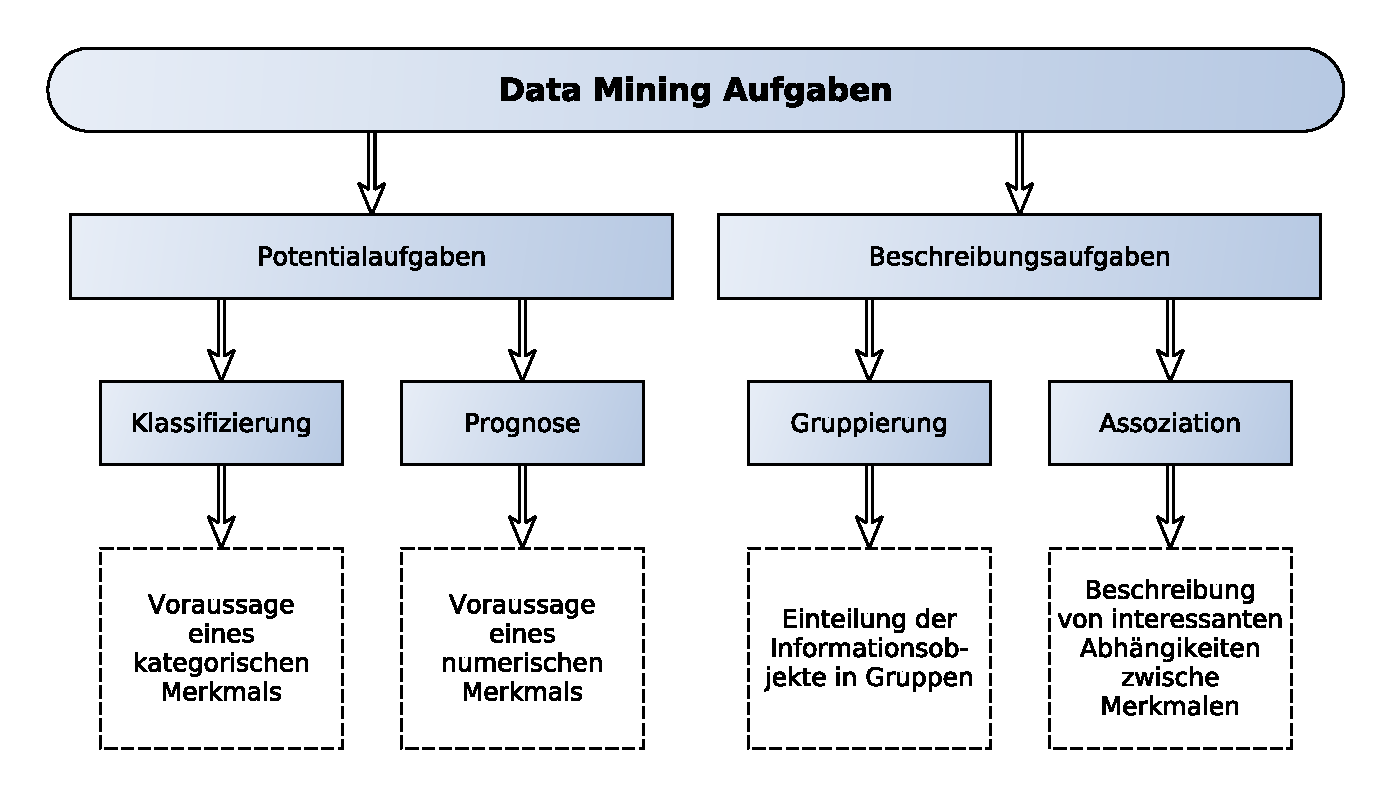
\includegraphics[width=\linewidth]{images/classification_data_mining_tasks.eps}
	\caption{Klassifizierung der Data Mining Aufgaben}
	\label{img:classification_data_mining_tasks}
\end{figure}

\subsection{Infrastruktur für künstliche Intelligenz im Onlinehandel}
Um dem Nutzer ein optimales Einkaufserlebnis zu ermöglichen, ist auch eine geeignete Infrastruktur erforderlich. Ein möglicher Ansatz ist in \cite{netz98_headless_commerce} und \cite{perske_headless_commerce} beschrieben. So können beispielsweise die Komponenten der künstlichen Intelligenz in einer Middleware, in der Abbildung \ref{img:infrastructor_for_ai_in_e__commerce} rot dargestellt integriert werden. Die Frontend-Anwendungen stellen eine Anfrage, zum Beispiel anzuzeigende "Produktempfehlungen" und erhalten die passenden Daten von der Middleware, die die Datensysteme abfragt. Daten können dann simultan aus verschiedenen Systemen geholt, verarbeitet und direkt an die jeweiligen Frontend-Anwendungen gesendet werden. Die verschiedenen Frontend-Anwendungen und Services sind unabhängig von den Datensystemen umgesetzt und verwenden die Daten und Funktionen der Datensysteme. Die Frontend-Anwendungen sind der Abbildung \ref{img:infrastructor_for_ai_in_e__commerce} gelb dargestellt und die Systemen mit den Datenquellen und Funktionalitäten sind grün.

\begin{figure}[!ht]
	\centering
	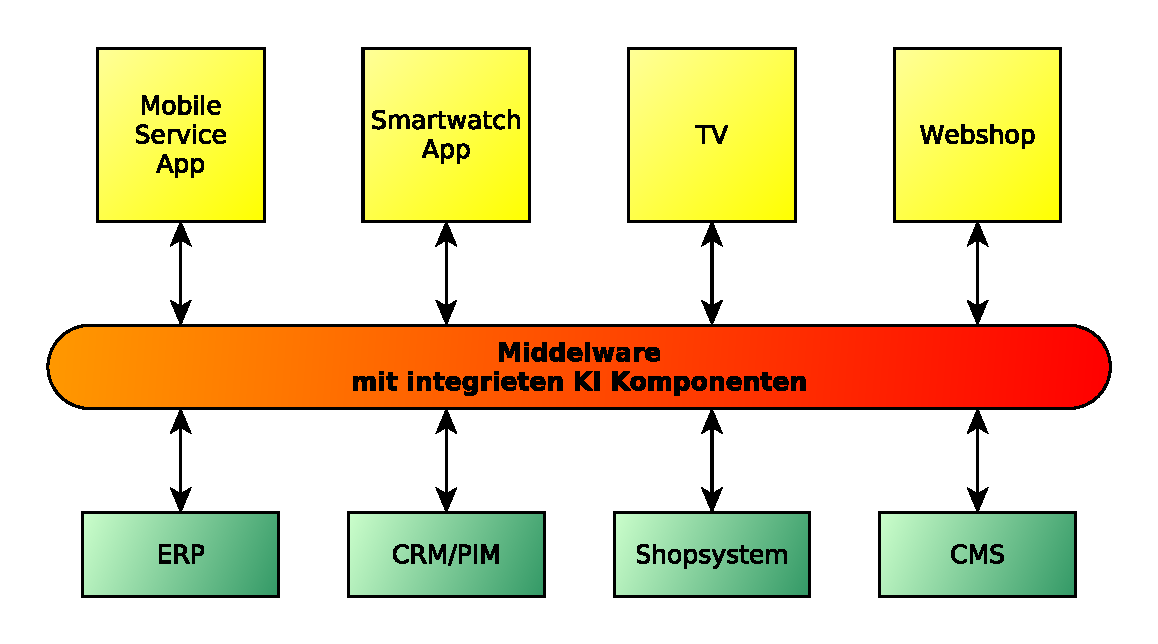
\includegraphics[width=\linewidth]{images/ecommerce-eco-system.eps}
	\caption{Mögliche Infrastruktur für künstlichen Intelligenz im Onlinehandel}
	\label{img:infrastructor_for_ai_in_e__commerce}
\end{figure}

\subsection{Prozesse der künstliche Intelligenz}
In \cite{glaess2018kuenstliche} auf Seite 3 werden die Einsatzgebiete von künstlicher Intelligenz im E-Commerce-Bereich in drei Bereiche gegliedert. In den folgen Abschnitte werden diese Bereiche näher besprochen und um einige Aufgaben erweitert. \cite{glaess2018kuenstliche} unterteilt die Bereiche in,

\begin{itemize}
	\item Planung \& Prozess,
	\item Produktangebot \& -darstellung und
	\item Beratung \& Service.
\end{itemize}

Die Abbildung \ref{img:areas_of_application_for_ai_in_e__commerce} zeigt eine grafische Zusammenfassung der verschiedenen Bereiche.

\begin{figure}[!ht]
	\centering
	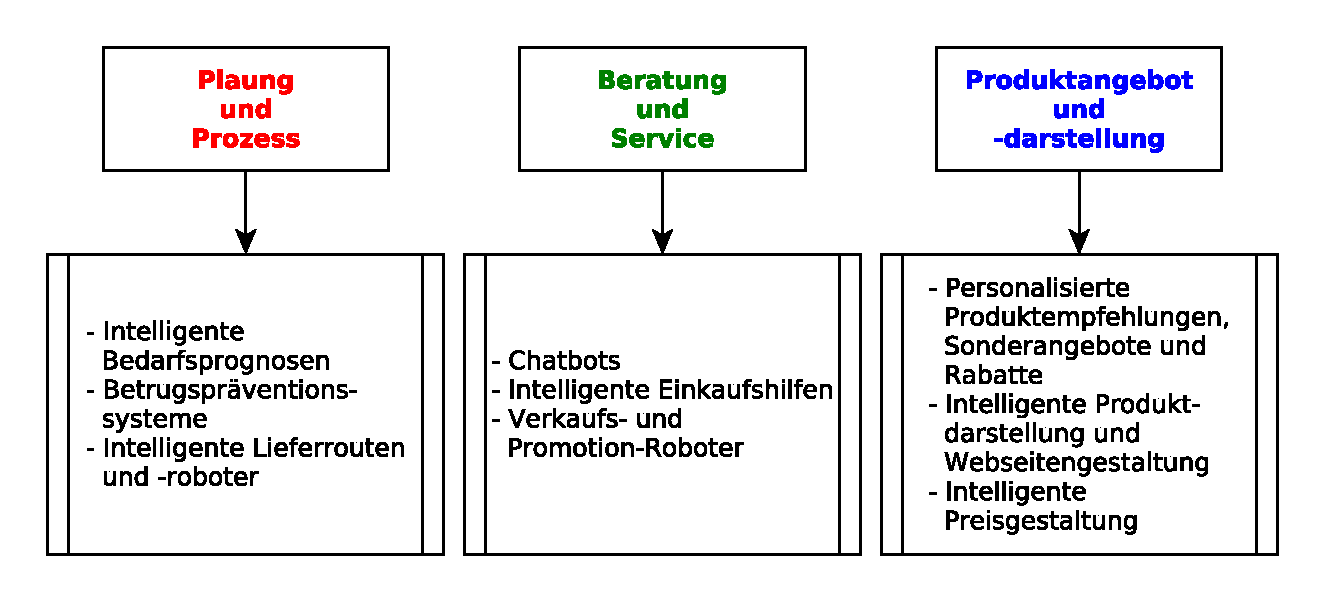
\includegraphics[width=\linewidth]{images/ki-bereiche_glaess.eps}
	\caption{Ansatzbereiche der künstlichen Intelligenz im Onlinehandel}
	\label{img:areas_of_application_for_ai_in_e__commerce}
\end{figure}

\subsubsection{Planung und Prozess}
\paragraph{Intelligente Bedarfsprognosen} erlauben die Optimierung der Bestellmengen und Automatisierung der Bestellprozesse, sodass Lagerbestände reduziert, Rücksendungen minimiert und Ressourcen effizienter werden können.\vspace{0.2cm}

In diesem Bereich sind die Aufgaben der Prognose erforderlich. So ist man in der Lage Trends zuerkennen und bei einer unbefriedigenden Bestandsentwicklung, können Maßnahmen ergriffen werden, um einer negativen Entwicklung des Bestandes entgegen zu wirken.\vspace{0.2cm}

Für die Optimierung wurden folgende Einflussfaktoren berücksichtigt,

\begin{itemize}
	\item Lagerbestand
	\item Lieferzeiten vom den Großhändlern
	\item prognostizierte Retouren
	\item Montagezeit des Produktes
	\item Preisentwicklung
\end{itemize}

Mit Hilfe der künstlichen Intelligenz wurden die Bestellungen bei den Großhändler prognostiziert und ausgelöst. So konnten Verkaufsspitzen im Vorfeld bearbeitet werden und es kann zu ca. 90\% weniger Lieferengpässen. Die Produktionszahlen konnten an die prognostizierten Verkaufszahlen angepasst werden und so verringert sich auch der Lagerbestand. Einerseits reduzierten sich die Bestände der Einzelteile die zur Fertigung benötigt wurden, anderseits die Bestände der produzierten Produkte. Bereits nach sechs Monaten wurden so die Lagerkosten um 10\% reduziert.\vspace{0.2cm}

Ein weiterer positiver Effekt waren die besseren Kundenbewertungen zu den Lieferzeiten im Online-Portal.

\paragraph{Betrugspräventionssysteme} entscheiden auf Basis von Verhaltens-, Zahlungs- und Produktdaten in Sekundenschnelle welche Zahlungsart einem Käufer angeboten werden und ermöglichen den beliebten Kauf auf Rechnung.\vspace{0.2cm}

Anhand von Verhaltensmuster, konnten mehr Betrugsversuche abgewendet werden. Dazu wurden bei auffälligem Verhalten weitere Verifikationen abgefragt und mit vorhandenen Daten verglichen. Beispielsweise wurde bei der Adresseingabe ein Abgleich mit einer Adressdatenbank durchgeführt und die Plausibilität der Daten gemessen. Wurde der Nutzer als großes Risiko eingestuft, wurde die Zahloption ,,Kauf auf Rechnung'' nicht angeboten.

\paragraph{Intelligente Lieferrouten und -roboter} berücksichtigen aktuelle Verkehrs- und Wetterdaten, um eine schnelle und zeitgenau Lieferung zum Kunden zu ermöglichen.
https://ecommerceinstitut.de/logistik-im-electronic-commerce/
Der Kunde hat die Möglichkeit seine bestellte Ware schnellst möglich oder zu einen selbstbestimmten Zeitpunk zu erhalten.\vspace{0.2cm}

Ebenfalls wurde bei der Lagerhaltung intelligente Robotik eingesetzt. Die Abbildung \ref{img:logistics_schema_in_e__commerce} zeigt ein Schema der Lagerverwaltung.

\begin{figure}[!ht]
	\centering
	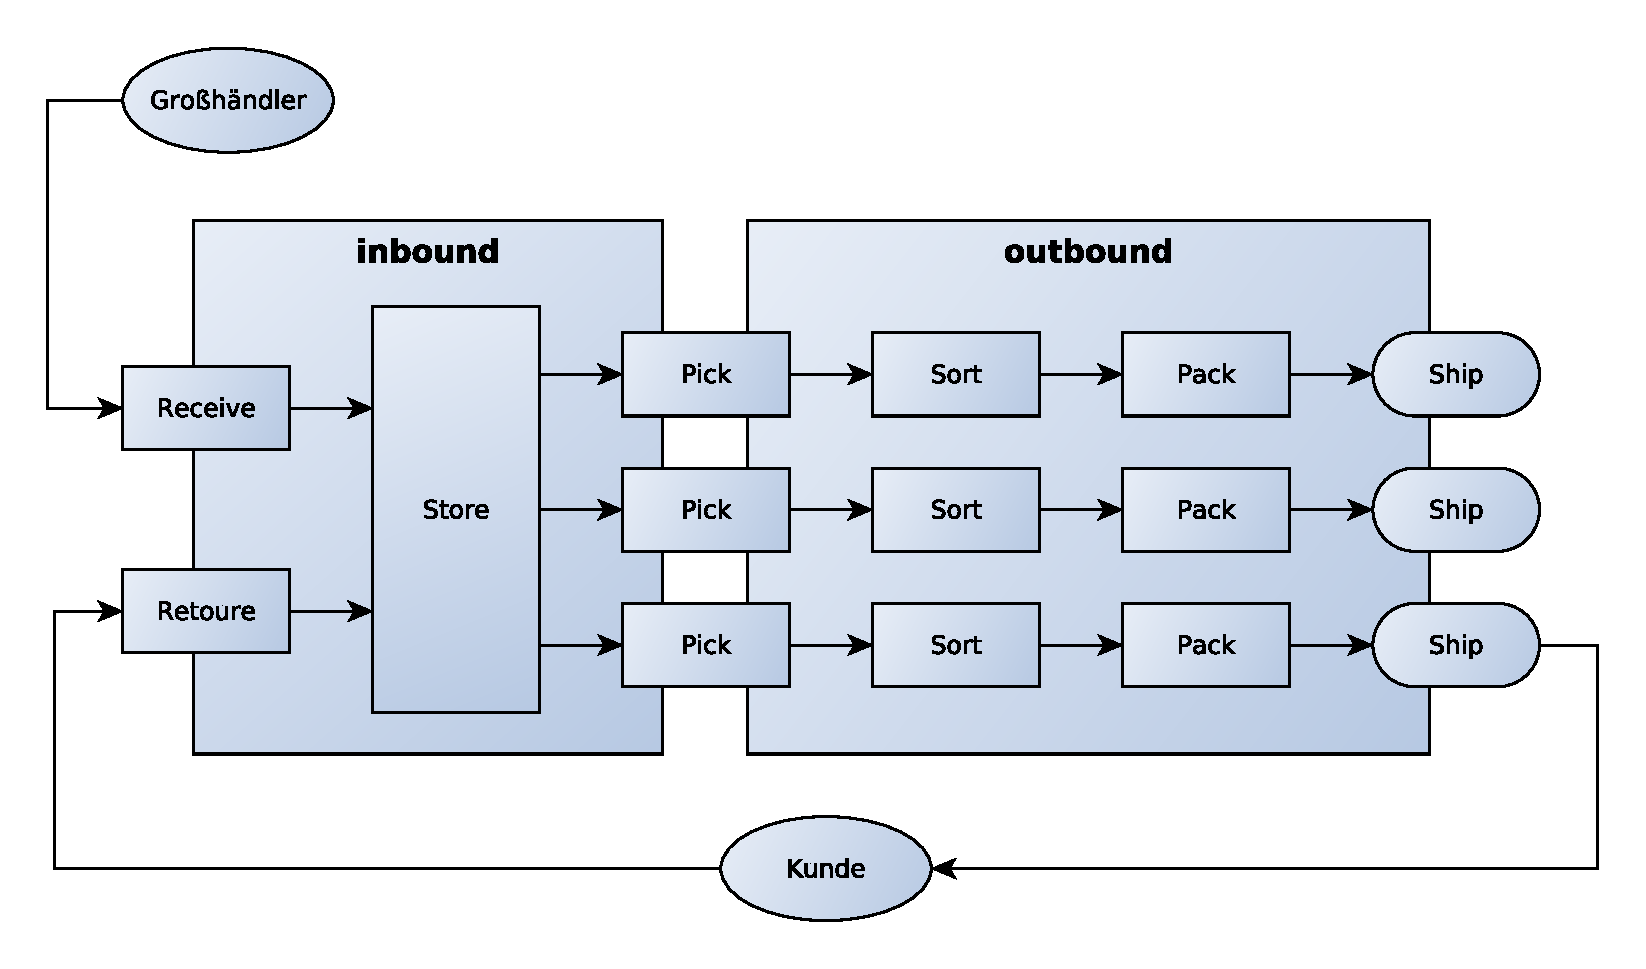
\includegraphics[width=\linewidth]{images/logistics-ecommerce.eps}
	\caption{Lagerhaltung mit künstlichen Intelligenz}
	\label{img:logistics_schema_in_e__commerce}
\end{figure}

Die Prozesse der Lagerwirtschaft beginnen mit der Lieferung vom Großhändler mit der Warenannahme, auch \textit{inbound} genannt. Hier erfolgt die digitale Erfassung der Waren.\vspace{0.2cm}

Im Anschluss werden diese in den sogenannten \textit{Store} eingelagert. Dabei wird auf den Ort der Einlagerung geachtet. Waren die in absehbarer Zeit mit häufigen Verkäufen zu rechnen ist, werden dicht an den Pick-Stationen einsortiert, um für die Pick-Roboter möglichst kurze Wege zu realisieren.\vspace{0.2cm}



Durch den Einsatz von intelligenter Robotik wurde das Hinzufügen und Entnehmen der Ware automatisiert, wodurch sich die Fehlerquote um fast 70 \% reduzierte.

\subsubsection{Produktangebot und -darstellung}
In diesem Bereich fällt alles, das mit Produkten und deren Preisbildung zu tun hat. Hierzu werden Nutzerverhalten und Kaufhistorien verwendet, um anhand von eine oder mehreren Merkmalen, möglichst homogene Kundensegmente zu erhalten. Diese Kundensegmente aus bestehenden und potenziellen Kunden kann eine intelligente Produktempfehlungen präsentiert werden.

\paragraph{Personalisierte Produktempfehlungen, Sonderangebote und Rabatte} berücksichtigen individuelle Wünsche und Bedürfnisse der Kunden und können so relevante Angebote ausspielen.\vspace{0.2cm}

Eine personalisierte Produktempfehlung kann anhand von vielen verschiedenen Parametern gemacht werden. Beispielsweise kann im Menü eine Unterteilung zwischen „Herren- und Damenmode“ erfolgen. So werden die jeweils anderen Produkte bereits zu beginn ausgeschlossen. Andere Merkmale der Kundenobjekte können ebenfalls für die Produktempfehlung herangezogen werden.\vspace{0.2cm}

Künstliche Intelligenz kann auch äußere Einflüsse bei der Produktempfehlung berücksichtigen. So können je nach Jahreszeit und Saison verschiedene Produkte Bevorzugt in den Fokus der Empfehlungen rücken.\vspace{0.2cm}

Neben den äußeren Einflussfaktoren, kann die künstliche Intelligenz auch die betrieblichen Faktoren berücksichtigen. Sind Artikel die sich schlechter Verkaufen lassen in großer Stückzahl im  Lagerbestand vorhanden, könnten diese zu besonderen Rabatten angeboten werden und somit die Lagerhaltungskosten senken. Auch können Kunden mit großen Warenkorbwert ein Rabatt gewährt werden, der Kunden mit niedrigen Warenkorbwert verwehrt bleibt.\vspace{0.2cm}

Sonderangebote können anhand der Daten ebenfalls durch die künstliche Intelligenz erstellt werden. So können Produkte die andere Kunden zusammen gekauft haben oder Produkte die ebenfalls angeschaut wurden zusammen als Produktbundel angeboten werden und mit den Hinweisen „Nutzer das kauften, kauften auch das“ oder „Nutzer die das kauften, sahen sich auch das an“ versehen werden.

\paragraph{Intelligente Produktdarstellung und Webseitengestaltung} stellt relevante Inhalte für den Kunden in übersichtlicher Weise dar, indem z.B. Produktbewertungen nach Themen gefiltert werden.\vspace{0.2cm}

Durch künstliche Intelligenz können Produktbeschreibung automatisch generiert werden. Dazu wird im Internet nach dem Produkten gesucht und individuelle Produktbeschreibungen erstellt. Oft mehrere Tausende pro Stunde. Der Vorteil ist das kostengünstig große Menge an Produktbeschreibungen bereitgestellt werden. So erhält jeder Kunde eine dynamisch-individuelle Produktbeschreibung.\vspace{0.2cm}

Mit Hilfe einer Textanalyse kann die künstliche Intelligenz relevante Informationen aus den Produktbeschreibungen der Hersteller extrahieren und die Produktbeschreibung besser an die Bedürfnisse der Kunden anpassen. So kann anhand der Kundenbedürfnisse und anhand der vorhandenen historischen Daten, eine personalisierte Produktempfehlung ausgegeben werden.\vspace{0.2cm}

Ebenfalls können die Kundenrezensionen in die Aufarbeitung der Produktbeschreibungen mit einfließen. Wird beispielsweise ein Artikel oft zurück gesandt, kann die Textanalyse bei  aus den Rezensionen eventuelle Fehlbeschreibungen ermitteln und diese korrigieren. Somit lässt sich die Retourenquote senken.\vspace{0.2cm}

Eine weitere Möglichkeit der Personalisierung ist die Optimierung der Webseite durch die künstliche Intelligenz. Dies kann bedeuten das einzelne Elemente wie Navigation, Anrede oder Produktempfehlung auf er Startseite personalisiert sind, aber auch, um eine barrierefreie Bedienung zu gewährleisten können Farben variieren oder Vorlesefunktionen integriert werden.

\paragraph{Intelligente Preisgestaltung} ermitteln den optimalen Preis unter Berücksichtigung von z.B. Wettbewerbspreisen, Wetterdaten und Lagerbeständen, um Lagerbestände zu reduzieren und Kostenunterschiede zu berücksichtigen.\vspace{0.2cm}

Hier kann künstliche Intelligenz helfen den optimalen Preis zu erzielen. Hierfür werden verschiedene Modelle verwendet, um zum richtigen Zeitpunkt den best möglichen Preis zu erzielen und dabei die Margen optimal zu halten. Zum Einsatz sind zwei Methoden, nach \cite{mckinsey_dynamic_pricing} gekommen.\vspace{0.2cm}

Zum einem das Key-Vauel-Item (KVI) Modell, bei der die Preiswahrnehmung von Verbraucher dynamisch ausgewertet wird. Dabei werden Daten aus dem Nutzerverhalten betrachtet, wie Klickrate, Suchdaten oder Produktbewertungen.\vspace{0.2cm}

Zum anderen mit dem reagieren auf die Bewegungen der Konkurrenz (Competitive-Response-Modell). Die Preisentwicklung der Wettbewerber wird dabei in Echtzeit überwacht und ggf. wird eine Preisanpassung der eigenen Preise durchgeführt.\vspace{0.2cm}

Ebenfalls werden höherwertige Produkte am Monatsanfang präsentiert und geringwertige Produkte am Monatsende. Auch Ortslokalisierung wird verwendet, um die Preise zu gestalten. So werden ebenfalls höherwertige Produkte angezeigt, wenn die Lokalisierung eine einkommensstarke Gegend ausweist.\vspace{0.2cm}

Ein weiterer Punkt ist die Berücksichtigung von saisonalen oder Trendprodukten. Diese werden in der Saison treuer angeboten, als in der Nebensaison. Ebenso Artikel die im aktuellen Trends liegen werden teurer angeboten, als solche Produkte, bei der zurzeit die Nachfrage gering eingeschätzt wird.

\paragraph{Zusammenfassung Produktangebot und Produktdarstellung} Kosten reduzieren und einsparen, sowie Umsatz steigern. Durch die personalisierte Gestaltung und personalisierten Angebote erhöht sich die Kundenbindungsrate um etwa 2\% und es entstand ein Traffic-Zuwachs. Ebenfalls erhöhte sich der Warenkorbwert um durchschnittlich 20\%. Die Kosten für den Lagerbestand verringerten sich um 14,5\%.\vspace{0.2cm}

Durch die intelligente Preisgestaltung konnte ein Umsatzwachstum von 6\% gesteigert und ein Margenzuwachs von 12\% erzielt werden.

\subsubsection{Beratung und Service}

Durch die Verbesserung des ,,Customer Journals'' konnte nochmals eine Umsatzsteigerung von 16\% erreicht werden, bei einer Kostensteigerung von etwa 2\% für neue Technologien.

\paragraph{Chatbots} bieten 24/7-Online-Kun\-den\-be\-ra\-tung und assistieren Mitarbeitern in Call-Center und Kundenchat, sodass Warteschlangen vermieden werden.\vspace{0.2cm}

Die Umsetzung des Chatbots wurde nach \cite{chatlogue_chatbot_tasks} gestaltet und wurde für die folgenden Einsatzmöglichkeiten konzeptioniert,

\begin{itemize}
	\item Informationsvermittlung,
	\item Vorqualifizierung von Kundenanfragen,
	\item Beantworten von wiederkehrenden Standardfragen,
	\item Beratung zu Produkten und
	\item Sendungsverfolgung
\end{itemize} 

Neben den eben genannten Vorteilen haben durch künstliche Intelligenz gestützte Bots weitere Vorteile,

\begin{itemize}
	\item Gleichzeitige Kommunikation mit mehreren Kunden,
	\item Lernen und aktualisieren sich selbstständig,
	\item erhöhen die Effizienz im Kundenservice, die Mitarbeiter können sich auf komplexere Anfrage konzentrieren,
	\item sinkende Fehlkäufe,
	\item verhindern Warenkorbabbrüche durch unerwartete Probleme,
	\item fördern Up- und Cross-Selling, da die Bots Empfehlungen aussprechen die zu den bereits im Warenkorb befindlichen Produkten passen,
	\item Mulit-Channel-Kommunikation die auf verschiedensten Endgeräten aufgeführt werden kann 
\end{itemize}

Durch die Einführung eines Chatbots auf der Webseite wurde, der Kundensupport deutlich verbessert, besonders außerhalb der Geschäftszeiten, dadurch erhöhte sich der Umsatzes, bei gleichzeitiger Verringerung der Fehlkäufe, einher gehend mit einer sinkenden Retourenquote.\vspace{0.2cm}

Zunächst kam der Bot bei der Produktberatung und bei Problemen im Checkout-Prozess zum Einsatz. Nach Initialisierungsphase mit einfachen und häufig vorkommenden Fragen, übernahm der Bot die Erstkommunikation mit dem Kunden. Beim Problemen wurde ein Agent aus dem Kundenservice hinzugezogen. Durch dessen Kommunikation mit dem Kunden wurde der Bote trainiert und übernahm nach und nach mehr Kommunikation ohne hinzuziehen eines Agenten. Nachdem der Bot die eingehende Frage zerlegt, analysiert und die relevante Fakten extrahiert hat, wird in der Datenbank und im Internet nach einer passenden Antwort gesucht und dem Nutzer bereitgestellt.\vspace{0.2cm}

Der Bot bekam zudem eigenes Nutzerprofil, dies bot dem Kunden den Anschein eine persönliche Betreuung.

\paragraph{Intelligente Einkaufshilfen} wie Alexa und Co. ermöglichen ein komfortables Einkaufserlebnis, indem sie bei der Einkaufsplanung unterstützen und den Kaufprozess vereinfachen.

\paragraph{Verkaufs- und Promotion-Roboter} unterstützen als digitale Verkäufer im stationären Geschäft z.B. bei der Navigation und Vorstellung von Produkten und Techniken.\vspace{0.2cm}

Die Daten die die künstliche Intelligenz für die Promotion 

Der Verkauf wurde von der künstlichen Intelligenz dahin gehend unterstützt, als das diese einfache Aufgaben erledigte. So übernahm diese bei nicht abgeschlossenen Warenkörben, nach drei Tagen die erneute Kommunikation mit dem Kunden.\vspace{0.2cm}

Ebenfalls wurden die mit einer Newsletter Aktion nach einem und drei Monaten erneut beworben und zwar mit Produkten für die sie sich interessierten und im Onlineshop angeschaut haben.\vspace{0.2cm}

Des weiteren wurden weitere Sales Promotionen eingeführt. Zu den eingeführten Maßnahmen zählen Aktionsverpackungen, Proben, Produktzugaben und ein Gewinnspiel. So wurden bei Bestellungen abhängig von den Produkten Proben von anderen Artikel mit versandt. Ebenfalls wurde für einen bestimmten Zeitraum Aktionspackungen mit größeren Stückzahlen oder als Produktkombination mit anderen Produkten angeboten. Durch ein Gewinnspiel konnten ca. weitere 1300 Neukunden gewonnen werden, welche einen zusätzlichen Umsatz von etwa 20000 \euro \, einbrachten.


	%A statement requiring citation \cite{Figueredo:2009dg}.
	
	%----------------------------------------------------------------------------------------
	%	REFERENCE LIST
	%----------------------------------------------------------------------------------------
	\bibliographystyle{ieeetr}
	\bibliography{content/bibliography}
	%\begin{thebibliography}{99} % Bibliography - this is intentionally simple in this template
		
	%	\bibitem[Figueredo and Wolf, 2009]{Figueredo:2009dg}
	%	Figueredo, A.~J. and Wolf, P. S.~A. (2009).
	%	\newblock Assortative pairing and life history strategy - a cross-cultural
	%	study.
	%	\newblock {\em Human Nature}, 20:317--330.
		
	%\end{thebibliography}
	
	%----------------------------------------------------------------------------------------
	
\end{document}